% Generated by code/ch13_qcpop_vs_grape.py -- do not edit by hand.
\definecolor{qocA}{rgb}{0.00,0.45,0.70}
\definecolor{qocB}{rgb}{0.90,0.60,0.00}
\definecolor{qocC}{rgb}{0.00,0.62,0.45}
\definecolor{qocD}{rgb}{0.80,0.40,0.00}
\definecolor{qocE}{rgb}{0.80,0.60,0.70}
\definecolor{qocF}{rgb}{0.35,0.70,0.90}
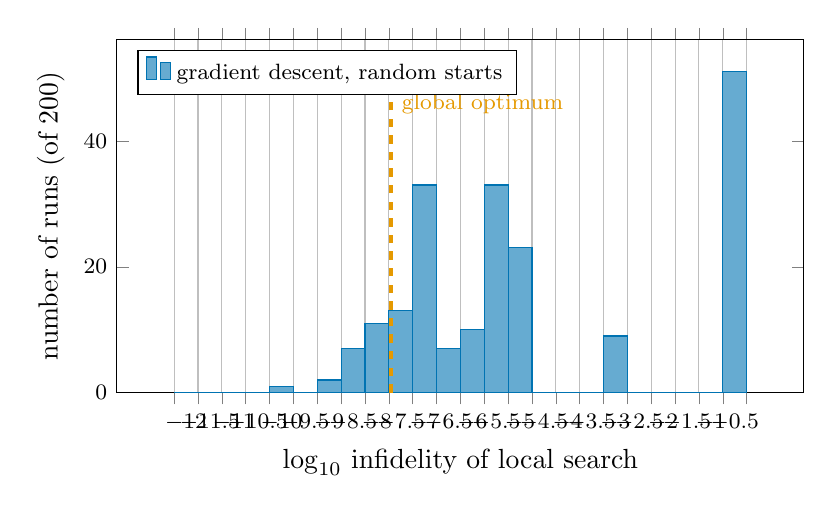
\begin{tikzpicture}[]
\begin{axis}[ybar interval, width=0.85\linewidth, height=0.5\linewidth,
  xlabel={$\log_{10}$ infidelity of local search}, ylabel={number of runs (of 200)},
  ymin=0, tick label style={font=\footnotesize}, legend style={font=\footnotesize}, legend pos=north west]
\addplot[fill=qocA!60, draw=qocA] coordinates {(-12.000,0) (-11.500,0) (-11.000,0) (-10.500,0) (-10.000,1) (-9.500,0) (-9.000,2) (-8.500,7) (-8.000,11) (-7.500,13) (-7.000,33) (-6.500,7) (-6.000,10) (-5.500,33) (-5.000,23) (-4.500,0) (-4.000,0) (-3.500,0) (-3.000,9) (-2.500,0) (-2.000,0) (-1.500,0) (-1.000,0) (-0.500,51) (0.000,51)};
\addlegendentry{gradient descent, random starts}
\draw[qocB, very thick, dashed] (axis cs:-7.455,0) -- (axis cs:-7.455,51) node[pos=0.9, right, font=\footnotesize] {global optimum};
\end{axis}
\end{tikzpicture}
